\begin{topic}{minkowski-theorem}{Minkowski's theorem}
    Let $L$ be a lattice in $\RR^n$, and $S \subset \RR^n$ a convex subset, which is symmetric with respect to the origin. That is, for all $x \in S$ also $-x \in S$. Then \textbf{Minkowski's theorem} states that if the volume of $S$ is strictly larger than $2^n \det(L)$, then $S$ must contain at least one non-zero lattice point of $L$.
\end{topic}

\begin{example}{minkowski-theorem}
    The given bound is sharp. Namely, consider $L = \ZZ^n$ with $\det(L) = 1$, and $S$ the interior of $[-1, 1]^n$, whose volume is $2^n$. Then $S$ does not contain any non-zero lattice points.
\end{example}

\begin{example}{minkowski-theorem}
    \begin{proof}
        By assumption, the set $\tfrac{1}{2} S = \{ \tfrac{1}{2} x : x \in S \}$ has volume $\textup{vol}(\tfrac{1}{2} S) = 2^{-n} \textup{vol}(S) > \textup{vol}(\RR^n/L)$, so the map $\tfrac{1}{2} S \to \RR^n / L$ cannot be injective. Hence, there are distinct points $x_1, x_2 \in S$ such that $\tfrac{1}{2} x_1 - \tfrac{1}{2} x_2 \in L$. Since $-x_2 \in S$ and $S$ is convex, the linear combination $\tfrac{1}{2} x_1 - \tfrac{1}{2} x_2$ is a non-zero lattice point in $S$.
    \end{proof}
\end{example}

\begin{topic}{root-system}{root system}
    Let $V$ be a finite-dimensional real or complex \tref{vector-space}{vector space} with an \tref{inner-product}{inner product} $\langle \cdot, \cdot \rangle$. A \textbf{root system} $\Phi$ in $V$ is a finite set of non-zero vectors in $V$, called \textbf{roots}, such that
    \begin{itemize}
        \item (\textit{span}) $\Phi$ spans $V$,
        \item (\textit{reduced}) if $\alpha \in \Phi$, then $n \alpha \in \Phi \iff n = \pm 1$,
        \item (\textit{reflection}) $\beta - \frac{2 \langle \alpha, \beta \rangle}{\langle \alpha, \alpha \rangle} \alpha \in \Phi$ for all $\alpha, \beta \in \Phi$,
        \item (\textit{integrality}) $\frac{2 \langle \alpha, \beta \rangle}{\langle \alpha, \alpha \rangle}$ is an integer for all $\alpha, \beta \in \Phi$.
    \end{itemize}
    Given a root system $\Phi$, one can always choose (non-uniquely) a subset $\Phi^+ \subset \Phi$ such that
    \begin{itemize}
        \item for all $\alpha \in \Phi$, either $\alpha \in \Phi^+$ or $-\alpha \in \Phi^+$, but not both,
        \item for distinct $\alpha, \beta \in \Phi^+$ such that $\alpha + \beta \in \Phi$, also $\alpha + \beta \in \Phi^+$.
    \end{itemize}
    Roots in $\Phi^+$ are called \textbf{positive} and roots in $-\Phi^+$ are called \textbf{negative}. An root in $\Phi^+$ is called \textbf{simple} (or \textbf{fundamental}) if it cannot be written as the sum of two positive roots. The set $\Delta$ of simple roots is called a \textbf{base} for $\Phi$ and has the property that every $\alpha \in \Phi$ is a linear combination of elements of $\Delta$ with integer coefficients, which are either all positive or all negative.
\end{topic}

\begin{example}{root-system}
    Given a complex \tref{AA:simple-lie-algebra}{semisimple Lie algebra} $\mathfrak{g}$ and a \tref{AA:cartan-subalgebra}{Cartan subalgebra} $\mathfrak{h} \subset \mathfrak{g}$, one can construct a root system $\Phi$ in $\mathfrak{h}^*$, where a root is an element $\alpha \in \mathfrak{h}^*$ such that
    \[ \mathfrak{g}_\alpha = \{ x \in \mathfrak{g} : [h, x] = \alpha(h) x \textup{ for all } h \in \mathfrak{h} \} \]
    is non-empty.
\end{example}

\begin{topic}{root-subsystem}{closed root subsystem}
    Let $(V, \Phi)$ be a \tref{root-system}{root system}. A \textbf{closed subsystem} of $(V, \Phi)$ is a subset $\Phi' \subset \Phi$ such that
    \begin{itemize}
        \item (\textit{subsystem}) if $\alpha, \beta \in \Phi'$, then $\beta - \frac{2 \langle \alpha, \beta \rangle}{\langle \alpha, \alpha \rangle} \alpha \in \Phi'$,
        \item (\textit{closed}) if $\alpha, \beta \in \Phi'$ and $\alpha + \beta \in \Phi$, then $\alpha + \beta \in \Phi'$,
        % \item (\textit{symmetric}) if $\alpha \in \Phi'$, then $-\alpha \in \Phi'$.
    \end{itemize}
    If $\Phi'$ only satisfies the second condition, it is simply called a \textbf{closed subset} of $(V, \Phi)$.
\end{topic}

\begin{topic}{weyl-group}{Weyl group}
    Let $\Phi$ be a \tref{root-system}{root system} in $V$. The \textbf{Weyl group} $W$ of $\Phi$ is the \tref{GT:subgroup}{subgroup} of the \tref{orthogonal-group}{orthogonal group} $\textup{O}(V)$ generated by the reflections
    \[ s_\alpha \colon V \to V, \quad v \mapsto v - 2 \frac{\langle v, \alpha \rangle}{\langle \alpha, \alpha \rangle} \alpha , \]
    for all $\alpha \in \Phi$. By definition of the root system, each $s_\alpha$ preserves $\Phi$, so $W$ is a finite group.
\end{topic}

\begin{example}{weyl-group}
    \begin{itemize}
        \item The Weyl group of the $A_n$ root system is the \tref{GT:symmetric-group}{symmetric group} $S_{n + 1}$.
    \end{itemize}
\end{example}

\begin{topic}{weyl-chamber}{Weyl chamber}
    Let $(V, \Phi)$ be a \tref{root-system}{root system}. The \textbf{Weyl chambers} of $(V, \Phi)$ are the connected components of the complement in $V$ of the union of all hyperplanes perpendicular to the roots $\alpha \in \Phi$.

    The \textbf{fundamental Weyl chamber} associated to a base $\Delta$ is the Weyl chamber
    \[ C(\Delta) = \{ v \in V \mid \langle \alpha, v \rangle > 0 \textup{ for all } \alpha \in \Delta \} , \]
    and conversely, every Weyl chamber $C$ determines a base
    \[ \Delta(C) = \{ \alpha \in \Phi \mid \langle \alpha, v \rangle > 0 \textup{ for all } v \in C \} . \]
\end{topic}

\begin{example}{weyl-chamber}
    Below is depicted the root system $A_2$. The dotted lines are the hyperplanes which are orthogonal to the roots. The filled area is one of the Weyl chambers, corresponding to the base $\Delta = \{ (0, 1), (\frac{1}{2} \sqrt{3}, -\frac{1}{2}) \}$.
    \[ \svg 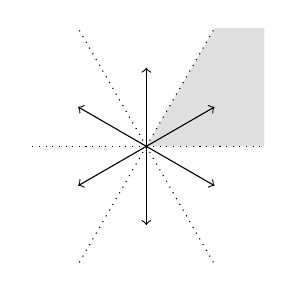
\begin{tikzpicture}
        \path[fill=gray!50, opacity=0.5] (0, 0) -- (0.866, 1.5) -- (1.5, 1.5) -- (1.5, 0);
        
        \draw[->] (0, 0) -- (0.866, 0.5);
        \draw[->] (0, 0) -- (0, 1);
        \draw[->] (0, 0) -- (-0.866, 0.5);
        \draw[->] (0, 0) -- (-0.866, -0.5);
        \draw[->] (0, 0) -- (0, -1);
        \draw[->] (0, 0) -- (0.866, -0.5);
        
        \draw[dotted] (0, 0) -- (1.5, 0);
        \draw[dotted] (0, 0) -- (-1.5, 0);
        \draw[dotted] (0, 0) -- (0.866, 1.5);
        \draw[dotted] (0, 0) -- (-0.866, 1.5);
        \draw[dotted] (0, 0) -- (0.866, -1.5);
        \draw[dotted] (0, 0) -- (-0.866, -1.5);
    \end{tikzpicture} \]
    Note that the \tref{weyl-group}{Weyl group}, in this case $W = S_3$, acts on the set of Weyl chambers (or equivalently, on the set of bases for $\Phi$). It is a theorem that this action is always free and transitive.
\end{example}

\begin{topic}{root-datum}{root datum}
    A \textbf{root datum} is a quadruple $(X^*, \Phi, X_*, \Phi^\vee)$, where
    \begin{itemize}
        \item $X_*$ and $X^*$ are \tref{GT:free-group}{free abelian groups} of finite rank, together with a perfect pairing $\langle \cdot, \cdot \rangle \colon X^* \times X_* \to \ZZ$,
        \item $\Phi \subset X^*$ and $\Phi^\vee \subset X_*$ are finite subsets with a bijection $\Phi \to \Phi^\vee, \alpha \mapsto \alpha^\vee$,
    \end{itemize}
    satisfying
    \begin{itemize}
        \item $\langle \alpha, \alpha^\vee \rangle = 2$ for all $\alpha \in \Phi$,
        \item $s_\alpha(\Psi) \subset \Psi$ and $s_{\alpha^\vee}(\Psi^\vee) \subset \Psi^\vee$ for all $\alpha \in \Psi$, where
        \[ \begin{aligned}
            s_\alpha &: X^* \to X^*, \quad x \mapsto x - \langle x, \alpha^\vee \rangle \alpha , \\
            s_{\alpha^\vee} &: X_* \to X_*, \quad x \mapsto x - \langle \alpha, x \rangle \alpha^\vee.
        \end{aligned} \]
        % \item the group of automorphisms of $X^*$ generated by the $s_\alpha$ is finite.
        % $\beta - \langle \beta, \alpha^\vee \rangle \alpha \in \Phi$ and $\beta^\vee - \langle \alpha, \beta^\vee \rangle \alpha^\vee \in \Phi^\vee$ for all $\alpha, \beta \in \Phi$.
    \end{itemize}
    The elements $\alpha \in \Phi$ are called the \textbf{roots} of the root datum, and $\alpha^\vee \in \Phi^\vee$ the \textbf{coroots}.
    
    A root datum is \textbf{reduced} if $2 \alpha \not\in \Phi$ for any $\alpha \in \Phi$.
\end{topic}

\begin{example}{root-datum}
    Let $G$ be a \tref{AG:reductive-algebraic-group}{reductive algebraic group} over an algebraically closed field $k$, with a split maximal torus $T$. Its root datum is the quadruple $(X^*, \Phi, X_*, \Phi^\vee)$, where
    \begin{itemize}
        \item $X^* = \Hom(T, \GG_m)$ is the character lattice,
        \item $X_* = \Hom(\GG_m, T)$ is the lattice of $1$-parameter subgroups,
        \item the perfect pairing $\langle \alpha, \lambda \rangle$ is given by taking the degree of the composition $\alpha \circ \lambda \colon \GG_m \to \GG_m$,
        \item the roots $\Phi$ are all non-zero $\alpha \in X^*$ for which
        \[ \mathfrak{g}_\alpha = \{ x \in \mathfrak{g} \mid \textup{Ad}_G(t) x = \alpha(t) x \textup{ for all } t \in T \} \]
        is non-zero, where $\mathfrak{g}$ denotes the Lie algebra of $G$,
        \item for each $\alpha \in \Phi$, it can be shown there exists a unique $\alpha^\vee \in X_*$ satisfying some sufficient conditions. This determines $\Phi^\vee$, and the bijection $\Phi \to \Phi^\vee$.
    \end{itemize}
    It is a theorem that for every reduced root datum, there exists up to isomorphism a unique split reductive algebraic group $G$ with that root datum.
\end{example}

\begin{example}{root-datum}
    % It can be shown that the bijection $\alpha \mapsto \alpha^\vee$ is uniquely determined.
    Since the axioms are symmetric, for any root datum $(X^*, \Phi, X_*, \Phi^\vee)$, the quadruple $(X_*, \Phi^\vee, X^*, \Phi)$ is also a root datum, called the \textbf{dual root datum}.
    % Namely, let $s_{\alpha^\vee} \colon X_* \to X_*$ be given by $\xi \mapsto \xi - \langle \alpha, \xi \rangle \alpha^\vee$, then
    % \[ \begin{aligned}
    %     \langle s_\alpha(\beta), s_{\alpha^\vee}(\beta^\vee) \rangle
    %         &= \langle \beta - \langle \beta, \alpha^\vee \rangle \alpha, \beta^\vee - \langle \alpha, \beta^\vee \rangle \alpha^\vee \rangle \\
    %             &= \langle \beta, \beta^\vee \rangle - \langle \beta, \alpha^\vee \rangle \langle \alpha, \beta^\vee \rangle (\langle \alpha, \alpha^\vee \rangle - 1 - 1) \\
    %             &= 2 ,
    % \end{aligned} \]
    % so it follows from uniqueness that $s_{\alpha^\vee}(\beta^\vee) = (s_\alpha(\beta))^\vee \in \Psi^\vee$.
\end{example}

\begin{topic}{root-lattice}{root lattice}
    The \textbf{root lattice} of a \tref{root-system}{root system} $(V, \Phi)$ is the $\ZZ$-module $Q = \ZZ \Phi \subset V$.
\end{topic}

\begin{topic}{weight-lattice}{weight lattice}
    Let $(V, \Phi)$ be a \tref{root-system}{root system}. An element $\mu \in V$ is \textit{integral} if $2 \frac{\langle \alpha, \mu \rangle}{\langle \alpha, \alpha \rangle}$ is an integer for all $\alpha \in \Phi$. The \textbf{weight lattice} of $(V, \Phi)$ is the $\ZZ$-module $P \subset V$ of all integral elements.
\end{topic}

\begin{example}{weight-lattice}
    The weight lattice $P$ is preserved under the \tref{weyl-group}{Weyl group}. Indeed, for any $\mu \in P$ and $\alpha \in \Phi$, the reflection $s_\alpha(\mu) = \mu - 2 \frac{\langle \mu, \alpha \rangle}{\langle \alpha, \alpha \rangle} \alpha$ satisfies
    \[ 2 \frac{\langle s_\alpha(\mu), \beta \rangle}{\langle \beta, \beta \rangle} = 2 \frac{\langle \mu, \beta \rangle}{\langle \beta, \beta \rangle} - \left( 2 \frac{\langle \mu, \alpha \rangle}{\langle \alpha, \alpha \rangle} \right) \left( 2 \frac{\langle \alpha, \beta \rangle}{\langle \beta, \beta \rangle} \right) \in \ZZ , \]
    for all $\beta \in \Phi$, so $s_\alpha(\mu)$ is integral as well.
\end{example}
